\documentclass[12pt]{article}
\usepackage[dvipsnames]{xcolor}
\usepackage{graphicx}
\usepackage{amsmath}
\usepackage{amssymb}
\usepackage[color,matrix,frame,arrow,curve]{xy}
\begin{document}


\begin{figure}[h!]
\centering
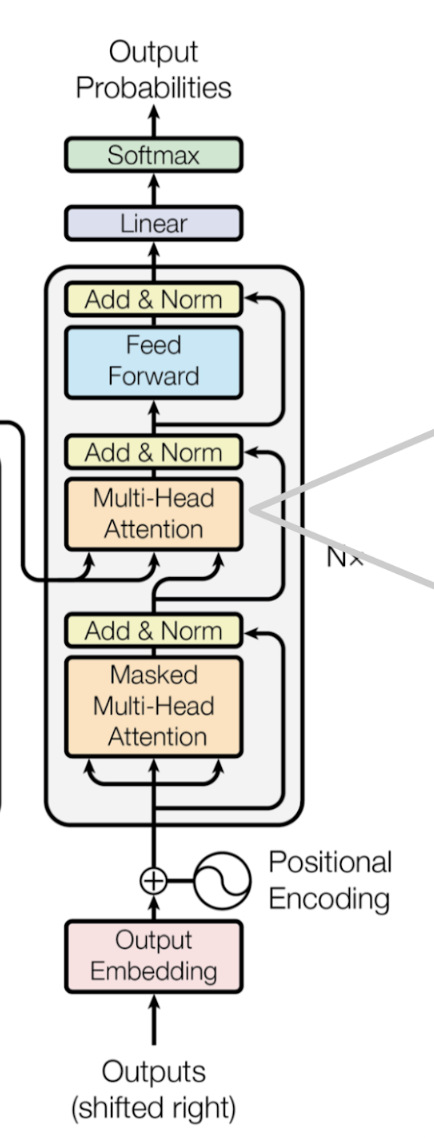
\includegraphics[width=2in]
{decoder.jpg}
\caption{View of Mount Vesuvius from
  Pompeii}
\label{fig-jpg}
\end{figure}


\begin{figure}[h!]\centering
$$\xymatrix{
&&&*+[F*:SpringGreen]{\underline{G}^{3\times  4}}
\\
&&&*+[F*:Orchid]{\underline{I}^{3\times  4}}\ar[u]
\\
&&&*+[F*:yellow]{\underline{Y}^{3\times  4}}\ar[u]
\\
&&*+[F*:SkyBlue]{\underline{B}^{3\times  4}}\ar[ur]&
\\
&&&*+[F*:yellow]{\underline{j}^{3\times  4}}
\\
*+[F*:Dandelion]{\underline{O}^{3\times  4}}\ar[urrr]&&&
\\
&&&*+[F*:yellow]{\underline{a}^{3\times  4}}\ar[uuuu]\ar[uuul]\ar[uu]\ar[ulll]
\\
&&*+[F*:Dandelion]{\underline{o}^{3\times  4}}\ar[ur]&
\\
&*+[F*:Dandelion]{\underline{Q}^{3\times  4}}\ar[ur]&*+[F*:Dandelion]{\underline{K}^{3\times  4}}\ar[u]&*+[F*:Dandelion]{\underline{V}^{3\times  4}}\ar[ul]
\\
&&&*+[F*:gray]{\underline{p}^{3\times  4}}\ar[uuu]\ar[ull]\ar[ul]\ar[u]
\\
*+[F*:Dandelion]{\underline{q}^{3\times  4}}\ar[uuuuu]&*+[F*:Dandelion]{\underline{v}^{3\times  4}}\ar[uuuuul]&&*+[F*:Lavender]{\underline{R}^{3\times  4}}\ar[u]
}$$
\caption{Decoder}
\label{fig-texnn-for-decoder}
\end{figure}\begin{subequations}
\begin{equation}
G^{3\times  4} = I^{3\times  4})
\label{eq-G-fun-decoder}
\end{equation}

\begin{equation}
I^{3\times  4} = Y^{3\times  4})
\label{eq-I-fun-decoder}
\end{equation}

\begin{equation}
Y^{3\times  4} = B^{3\times  4},a^{3\times  4})
\label{eq-Y-fun-decoder}
\end{equation}

\begin{equation}
B^{3\times  4} = a^{3\times  4})
\label{eq-B-fun-decoder}
\end{equation}

\begin{equation}
j^{3\times  4} = O^{3\times  4},a^{3\times  4})
\label{eq-j-fun-decoder}
\end{equation}

\begin{equation}
O^{3\times  4} = q^{3\times  4},v^{3\times  4},a^{3\times  4})
\label{eq-O-fun-decoder}
\end{equation}

\begin{equation}
a^{3\times  4} = o^{3\times  4},p^{3\times  4})
\label{eq-a-fun-decoder}
\end{equation}

\begin{equation}
o^{3\times  4} = Q^{3\times  4},K^{3\times  4},V^{3\times  4})
\label{eq-o-fun-decoder}
\end{equation}

\begin{equation}
Q^{3\times  4} = p^{3\times  4})
\label{eq-Q-fun-decoder}
\end{equation}

\begin{equation}
K^{3\times  4} = p^{3\times  4})
\label{eq-K-fun-decoder}
\end{equation}

\begin{equation}
V^{3\times  4} = p^{3\times  4})
\label{eq-V-fun-decoder}
\end{equation}

\begin{equation}
p^{3\times  4} = R^{3\times  4})
\label{eq-p-fun-decoder}
\end{equation}

\begin{equation}
R^{3\times  4} =)
\label{eq-R-fun-decoder}
\end{equation}

\begin{equation}
q^{3\times  4} =)
\label{eq-q-fun-decoder}
\end{equation}

\begin{equation}
v^{3\times  4} =)
\label{eq-v-fun-decoder}
\end{equation}

\end{subequations}


\end{document}  
